\documentclass{article}
\usepackage{algpseudocode,algorithm,algorithmicx}
\usepackage[usenames,dvipsnames,svgnames,table]{xcolor}
\usepackage{hyperref}
\usepackage{graphicx}
\begin{document}
    \title{\textcolor{blue}{\textbf{Problema 4 }}\\}
    \author{Daniel de la Cruz Prieto C211\\ David Orlando De Quesada Oliva C211\\Javier Dominguez C212} 
    \date{}
    \maketitle  

    \section{Orden del problema} 
    Sea $G = <V, E>$ un grafo no dirigido y conexo, se desea saber si G cumple la propiedad de que cada par de
    v\'ertices existen dos caminos disjuntos en v\'ertices entre ellos. La complejidad temporal de su algoritmo debe
    ser $O(|V| + |E|)$.
    \newline
    \newline
    \section{Soluci\'on} 
    Lema 1:\newline
    $\forall x,y\in V(G)$ existen dos caminos disjuntos en v\'ertices $\Longleftrightarrow$ G es biconexo \newline
    \newline
    Demostraci\'on:\newline
    $\Longrightarrow$\newline
    Sea x un v\'ertice arbitrario de G. En el grafo G-x(resultado de remover el v\'ertice x del grafo G)
    sigue habiendo un camino entre cualquier par de v\'ertices u,v pues como en G existen dos caminos disjuntos en v\'ertices
    entre u y v si x pertenec\'ia a uno de estos dos caminos no importa pues al removerlo sigue habiendo al menos un camino 
    entre u y v por lo que G-x ser\'ia conexo. Entonces al remover cualquier v\'ertice de G y todas las aristas incidentes a
    \'el no desconectan el grafo . Luego G es biconexo.\newline
    $\Longleftarrow$\newline
    Sea G un grafo biconexo y u,v v\'ertices del mismo.Vamos a demostrar por inducci\'on en la distancia $d(u,v)$ que hay
    dos caminos disjuntos en v\'ertices de u a v $\forall u,v \in V(G)$.
    \newline
    Caso Base $d(u,v)=1$:\newline
    Si $d(u,v)=1$ entonces la arista $<u,v>$ es uno de los caminos que conectan a u con v.Como G es biconexo entonces 
    G-u y G-v son conexos y por tanto si quitas la  arista $<u,v>$  como el grafo no se desconecta sigue existiendo
    un camino que conecta a u con v y que no contiene a $<u,v>$ ,este ser\'ia nuestro segundo camino.\newline
    
    \noindent \textbf{Paso Inductivo:}\\
    \begin{figure}[H]
        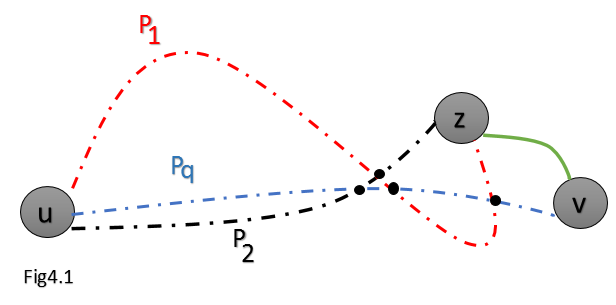
\includegraphics[scale = 0.327]{4fig1.png}
        \centering
    \end{figure}
    \noindent Sea G un grafo donde $\forall\; u,v\in V(G)\; d(u,v)=k>1$. Entonces en G existe un camino de longitud k entre 
    cualquier par de v\'ertices u,v.Sea z el \'ultimo v\'ertice anterior a v en el camino de de longitud k que va de
    u a v .Obtenemos $d(u,z)=d(u,v)-1=k-1$ . Por hip\'otesis de inducci\'on existen dos caminos disjuntos en v\'ertices 
    $P_{1},P_{2}$ de u a v.Dado que G-z es conexo pues G es biconexo ,entonces existe un camino $P_{q}$ que va de u a v
    y no contiene a z.Si $P_{q}$ no intercepta con $P_{1}$ o con $P_{2}$,tenemos los dos caminos disjuntos en v\'ertices
    de u a v:$P_{q}$ y $P_{1}$ o $P_{2}$(uno de los 2 con el que no tiene intercepci\'on) + $<u,v>$.Si $P_{q}$ intercepta 
    con $P_{1}$ y con $P_{2}$ vamos a crear un camino que comienza en v sigue por $P_{q}$ hasta la primera intercepci\'on con
    $P_{1}$ o $P_{2}$ y sigue por uno de estos dos hasta u,este camino no contiene a z. Ahora creamos  otro camino que vaya 
    desde u, por el camino que que no tomamos entre $P_{1}$ y $P_{2}$ en el camino previamente construido,  hasta z y con la arista $<z,v>$ llega 
    a v. Encontramos dos caminos disjuntos en v\'ertices que van de u a v$(fig4.1)$.\newline
    Luego en G hay dos caminos disjuntos en v\'ertices de u a v $\forall u,v \in V(G)$
    \newline
    \newline
    Lema 2:\newline
    G es biconexo $\Longleftrightarrow$ G no tiene puntos de articulaci\'on \newline
    Demostraci\'on:\newline
    $\Longrightarrow$\newline
    Si G es biconexo entonces al quitar cualquier v\'ertice v de G y las aristas incidentes al mismo 
    G sigue siendo conexo por lo no se divide en 2 o m\'as de componentes conexas .Por tanto G no
    tiene puntos de articulaci\'on.\newline
    $\Longleftarrow$\newline
    Si G no tiene puntos de articulaci\'on entonces no existe ning\'un  v\'ertice v que quite de G que lo separe en
    2 o m\'a  componentes conexas.Entonces G-v sigue siendo conexo.Luego G es biconexo.
    \newline
    \newline
    Lema 3:\newline
    $\forall x,y\in V(G)$ existen dos caminos disjuntos en v\'ertices $\Longleftrightarrow$ G no tiene puntos de articulaci\'on\newline
    Demostraci\'on:\newline
    Por Lema1  $\forall x,y\in V(G)$ existen dos caminos disjuntos en v\'ertices $\Longleftrightarrow$ G es biconexo. 
    Por Lema2 G es biconexo $\Longleftrightarrow$ G no tiene puntos de articulaci\'on.
    Entonces por transitividad $\forall x,y\in V(G)$ existen dos caminos disjuntos en v\'ertices 
    $\Longleftrightarrow$ G no tiene puntos de articulaci\'on
    \newline
    \newline
    \newline
    \section{Correctitud} 
    Correctitud del problema:
    \newline
    Por lo expuesto con anterioridad en los lemas 1,2 y 3 y por la correctitud del algoritmo de detecci\'on de puntos de 
    articulaci\'on, podemos asegurar la correctitud de nuestro algoritmo para detectar si un grafo G cumple la propiedad 
    de que cada par de v\'ertices existen dos caminos disjuntos en v\'ertices entre ellos, o sea con almacenar en una lista
    los puntos de articulaci\'on detectados por el algoritmo y verificar si la lista contiene alg\'un v\'ertice es suficiente.
    La modificaci\'on al algoritmo visto en conferencia es, en vez de imprimir el punto de articulaci\'on, simplemente lo
    almacenamos en una lista, lo que no afecta la correctitud del algoritmo. 
    \newline

    \section{Complejidad Temporal} 
    Complejidad Temporal:\newline
    La complejidad temporal de nuestro algoritmo es la complejidad temporal del algoritmo de detecci\'on de puntos 
    de articulaci\'on que es $O(|V|+|E|)$.La modificaci\'on que hicimos del c\'odigo de conferencia no afecta la 
    complejidad del algoritmo pues solo cambia imprimir el v\'ertice por agregar el v\'ertice a la lista que es una
    operaci\'on $O(1)$.Luego preguntar por el size de la lista para saber si se encontraron puntos de articulacici\'on 
    es O(1) por lo que sigue siendo $O(|V|+|E|)$ la complejidad de mi algoritmo.
    \newline
    
    \section{Pseudoc\'odigo}
    
    \begin{algorithm}[H] 
        Pseudoc\'odigo:
        \caption{Determinar si un grafo G cumple $\forall x,y\in V(G)$  existen dos caminos disjuntos en v\'ertices de x a y }
        \textbf{Solve($G$)\\}
        $answer=[\;]$ -lista para almacenar los puntos de articulaci\'on\\
        $childrens=[\;]$- array para saber cuantos hijos un v\'ertice que pertenece al \'arbol resultado de hacer DFS-Visit\\
        1-\hspace*{1em}DFS-Visit-PA($G,u$) \\ 
        2-\hspace*{2em}u $\leftarrow$ visited \\
        3-\hspace*{2em}$time=time+1$ \\
        4-\hspace*{2em}$d[u]=tome$\\
        5-\hspace*{2em}$low[u]=d[u]$\\ 
        6-\hspace*{2em}for each v $\in$ $Adj[u]$\\
        7-\hspace*{3em}do if v not visited\\
        9-\hspace*{4em}$\pi[v] \leftarrow u$\\
        9-\hspace*{4em}$childrens[u] \leftarrow childrens[u]+1$\\
        10-\hspace*{4em}DFS-PA(G)\\
        11-\hspace*{4em}$low[u]=min(low[u],low[v])$\\
        12-\hspace*{4em}if $low[v]\ge d[u]$\\
        13-\hspace*{5em}answer.add(u)\\
        14-\hspace*{3em}else if $pi[u]\ne v$\\
        15-\hspace*{4em}$low[u]=min(low[u],d[v])$\\ 
        15-\hspace*{2em}return\\\\
        17-\hspace*{1em}DFS-PA($G$)\\
        18-\hspace*{2em}for each v $\in$ V(G)\\
        19-\hspace*{3em}do if not visited\\
        22-\hspace*{4em}DFS=DFS-Visit-PA(G,v)\\
        20-\hspace*{4em}if $childrens[v] \ge 2$ -en caso de que la ra\'iz v de ese \'arbol de DFS sea art point \\
        21-\hspace*{5em}anwser.add(v)\\
        24-\hspace*{2em}return \\\\
        25-\hspace*{1em}ArtPoint($G$)\\
        25-\hspace*{2em}DFS-PA($G$)\\
        26-\hspace*{2em}if $size(anwser) >0$\\
        27-\hspace*{3em}return False\\
        28-\hspace*{2em}else\\
        29-\hspace*{3em}return True\\
        
        %Me parece que seria mejor si lo agrego a una lista y despues pregunto por lista.count para no modificar mucho del codigo
        
    \end{algorithm}

\end{document}